%% This is an example first chapter.  You should put chapter/appendix that you
%% write into a separate file, and add a line \include{yourfilename} to
%% main.tex, where `yourfilename.tex' is the name of the chapter/appendix file.
%% You can process specific files by typing their names in at the 
%% \files=
%% prompt when you run the file main.tex through LaTeX.
\chapter{Implementation}

\section{Cyclic Reduction}
Cyclic reduction (CR) is an algorithm introduced by G. H. Golub and R. W. Hoekney [26] in the mid 1960s for solving tridiagonal linear systems related to the finite difference discretization of the Poisson equation over a rectangle. 
The basic idea of the CR algorithm , also called odd-even reduction, is to repeatedly reduce the system to half size until one equation is left and solve backwards to find all unknowns. 
\subsection{The algorithm}
CR method only applies to matrices that can be represented as a (block) Toeplitz matrix; such problems often arise in implicit solutions for partial differential equations on a grid. For example fast solvers for Poisson's equation express the problem as solving a tridiagonal matrix, discretising the solution on a regular grid. From 1D Poisson’s equation arises a tridiagonal matrix system while from 2D Poisson’s equation arises a block tridiagonal system.
In general large tridiagonal systems of linear equations appear in many numerical analysis applications. A tri-diagonal matrix is a matrix with values only in the sub-, main- and super-diagonal.
For example, the tridiagonal system:\\
$a_i*x_{i-1} + b_i*x_i+c_i*x_{i+1} = F_{i}$  , \hspace*{2cm} $ i=1:1:n$\\

Assume that $n= 2^p - 1$. 
The algorithm proceeds in two steps: a forward reduction and a backward substitution. Each phase consists of ($\log_2n – 1$) steps, where n is the system size. The first step in cyclic reduction is to combine linearly the equations in order to eliminate the odd numbered unknowns ($x_1$, $x_3$ … $x_n$). Next the unknowns are re-ordered and the process is continued until the system consists from one equation with one unknown. To do this the algorithm is based to triplets. In the above example in order to eliminate $x_1$ and $x_3$,the first three equations of the system are chosen and multiplied by the parameters $\alpha_2$, $\beta_2$, $\gamma_2$. \\
\\
$b_1*x_1+c_1*x_2= F_1$                        \hspace*{5cm} $*(\alpha_2)$	\\
$a_2*x_1+ b_2*x_2+c_2*x_3= F_2$               \hspace*{3,3cm} $* (\beta_2)$  \\
\hspace*{2cm}$a_3*x_2+ b_3*x_3+c_3*x_4= F_3$  \hspace*{1,3cm} $*(\gamma_2)$     \\ \\

Subsequently the equations are summed and the resulted equation is produced. Similarly, this elimination process proceeds for the next three equations, until only one equation left.
Using the back substitution the unknown x can be calculated from the last one equation and  all the others $x_i$ can be found  from the previous steps .
The equations involved in all these stages are:\\\\
$a'_i = -a_{i-1} *k_1$\\
$b'_i = b_{i} - c_{i-1}*k_1 - a_{i+1} *k_2$\\
$c'_i = -c_{i+1} *k_2$\\
$d'_i = d_{i} - d_{i-1}*k_1 - d_{i+1} *k_2$\\
where $k_1 = \frac{a_i}{b_{i-1}} , k_2 = \frac{c_i}{b_{i+1}} $\\
$x_i = \frac{d'_i - a'_i * x_{i-1} - c'_i * x_{i+1}}{b'_i}$\\
\newpage
The described steps can be illustrated in Figure 4-1.
\begin{figure}[H]
   \centering
       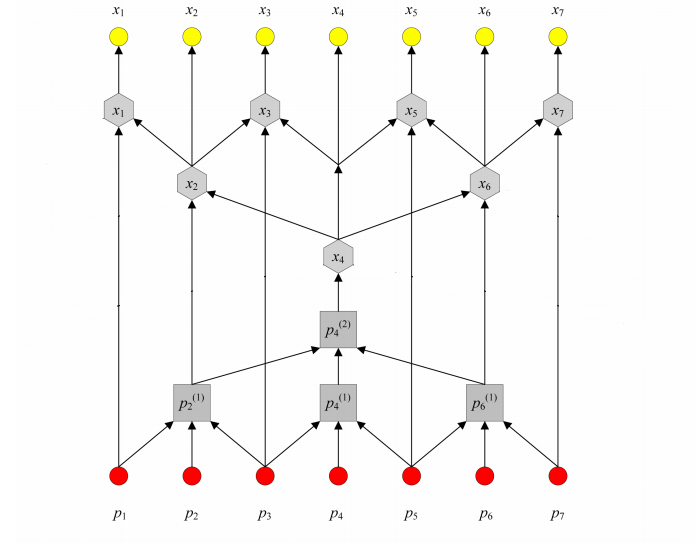
\includegraphics[width=0.5\textwidth]{figures/cr}
   \caption{CR Method}
   \label{fig:cr}
\end{figure}
%\newpage
\subsection{Implementation Issues}
As it was said a tridiagonal matrix has basically 3 diagonals, (super, main, sub). To take advantage of this, only these three diagonals vectors plus one vector for the right hand side of the system and one vector for the solution have to be stored.
Vectors a, b , c are used to hold the  sub-diagonal, the main diagonal and the super-diagonal respectively. Vector F holds the right hand side and U the solution vector. The code implemented for all the steps of the algorithm is given below: \\
\begin{algorithm}[H]
\begin{algorithmic}[1]
\Function{Forward Reduction}{}
\State{for$(i=0;  i<\log_2(size+1)-1; i++)$\{}
	 \State{\hspace*{1cm}for$(j=2^{i+1}-1; j<size; j=j+2^{i+1})$\{}
	    \State{\hspace*{2cm}$offset = pow(2,i);$}
        \State{\hspace*{2cm}$index_1=j-offset;$}        
        \State{\hspace*{2cm}$k_1 = a[j]/b[index_1];$}
        \State{\hspace*{2cm}$k_2 = c[j]/b[j];$}
        \State{\hspace*{2cm}$b[j] = b[j] - c[j-offset] * k_1 - a[j+offset] * k_2;$}
        \State{\hspace*{2cm}$F[j] = F[j] - F[j-offset] * k_1 - F[j+offset] * k_2;$}
        \State{\hspace*{2cm}$a[j] = -a[j-offset] * k_1;$}
        \State{\hspace*{2cm}$c[j] = -c[j+offset] * k_2;$}
        \State{\hspace*{2cm}\}}
      \State{\}} 
\EndFunction
\end{algorithmic}
\caption{Cyclic Reduction - Forward}
\label{alg:forward_cr}
\end{algorithm}
After the forward elimination the resulting system is one equation with one unknown. Hereafter, it is trivial to deduce the middle unknown of the system. 
\begin{algorithm}[H]
\begin{algorithmic}[1]
\Function{Find middle}{}
\State{$int index = (size-1)/2;$} 
\State{$x[index] = F[index]/b[index];$} 
\EndFunction
\end{algorithmic}
\caption{Solve the middle equation}
\label{alg:Find middle}
\end{algorithm}
Afterwards, the algorithm backwards to calculate repeatedly the remaining unknowns. Substantially, the resulting solution is calculated by the following code:
\begin{algorithm}[H]
\begin{algorithmic}[1]
\Function{Backward Substitution}{}
\State{for$(i=\log_2(size+1)-2;i>=0;i--)$\{ }
	 \State{\hspace*{1cm}for$(j=2^{i+1}-1;j<size;j=j+2^{i+1})$\{ }
	    \State{\hspace*{2cm}$offset = 2^i;$}
        \State{\hspace*{2cm}$index_1 = j-offset;$}        
        \State{\hspace*{2cm}$index_2 = j+offset;$}        
        \State{\hspace*{2cm}$if(j!=index_1)$}
       		\State{\hspace*{3cm}$ x[index_1] = (F[index_1] - a[index_1]*x[index_1-offset] - c[index_1]*x[index_1+offset])/b[index_1];$}
        \State{\hspace*{2cm}$if(j!=index_2)$}
        	\State{\hspace*{3cm}$x[index_2] = (F[index_2] - a[index_2]*x[index_2-offset] - c[index_2]*x[index_2+offset])/b[index_2];$}    
        	\State{\hspace*{2cm}\}}
        	\State{\}} 
\EndFunction
\end{algorithmic}
\caption{Cyclic Reduction - Backward}
\label{alg:Backward_cr}
\end{algorithm}
The first attempt was to simply port the above algorithm on GPU. Initially three kernels were obtained based on the three independent steps (Forward Reduction, Find middle, Backward Substitution) shown above. 
At this point, data dependencies were observed  between iterations of the external loop both in Forward Reduction kernel and in Backward Substitution kernel. Subsequently, the first Kernel for forward elimination called in this way:

\begin{lstlisting}[frame=single]
for (i=0;i<log2(size+1)-1;i++){
 <Kernel forward launch>
}
\end{lstlisting}

Variable i holds the iteration of the loop and passes as parameter in the kernel, which essentially settles on the termination condition.In a symmetric way the  Backward Substitution kernel is launched, but with the iterations in decreasing order.
The kernel Find middle is launched by one thread only, since is it actually one computation.
One essential optimization that was performed and increased significantly the speed up, as is will be shown in chapter five, is the dynamic calculation of the block dimension.It was observed that according to the iterations of the external loop, the number of the threads actually doing a job, was affected. So it was considered the following function in order to modify the size of the block dynamically:
\begin{algorithm}[H]
\begin{algorithmic}[1]
\Function{Calculate Block Dimension}{size,block,grid}
\State{if$(size<4)$\{$block->x=1;block->y=1;$\}}
\State{else if$(size<16)$\{$block->x=2;block->y=2;$\}}
\State{else if$(size<64)$\{$block->x=4;block->y=4;$\}}
\State{else if$(size<256)$\{$block->x=8;block->y=8;$\}}	
\State{else \{$block->x=16;block->y=16;$\}}
\EndFunction
\end{algorithmic}
\caption{Block Dimension}
\label{alg:calc_dim}
\end{algorithm}
In other words, the geometry changes while the size of the system is growing. 
Likeness for the backward substitution step, the block dimension is determined.

Another optimization considered was padding. Padding is a technique often used to avoid divergence between threads in a warp, caused mainly by branches. This technique is implemented by increasing the allocated memory in order to eliminate the branches.
In this implementation, padding was used to remove the if - branches in Backward Substitution kernel. These if - branches were present to preserve that threads would not exceed the allocated memory size. The maximum offset that threads could exceed was $\log_2(size+1)$ . So the padded vectors was $2*\log_2(size+1)$ bigger in order to cover both directions.
Performance results are demonstrated in Chapter 5.

In relation to memory transfers, before the kernels launches, all vectors except vector U are transferred from host to device using continuous CudaMemcpy(). It was preferred to initialize to zero the resulting vector U using CudaMemSet() instead of copying it through CudaMemcpy() due to lower cost. Finally, the only vector which is necessary to be copied back from the device to host is the solution vector U.
\section{Block Cyclic Reduction}
The basic idea of the cyclic reduction method can be extended to block tridiagonal systems. The idea of the block cyclic reduction (BCR) was first introduced by Gene Golub to deal with the scalar tridiagonal systems that arise from the finite element discretization of the Poisson equation in 2D. As in cyclic reduction, block cyclic reduction is a two phase algorithm. It consists of forward reduction and backward substitution. During each step of the reduction stage, are eliminated approximately half the unknowns in the system. After $O(\log_2 (n+1))$ reductions a $1x1$ block system is left. After solving this system, the previously eliminated unknowns are computed by back substitution. While this formulation is numerically unstable, O.Buneman suggested a stable variation[].  In this thesis, we consider the case of block cyclic reduction, where the scalar elements of traditional cyclic reduction are replaced with matrix tridiagonal and diagonal blocks.
\subsection{The algorithm}
The implemented algorithm solves systems of the following form:
 $A*U = F$\\  
where the \emph{A} is a block tridiagonal matrix: 
\[ \left( \begin{array}{ccccc}
B  & T &     &   &\\
T  & B &  T  &    &\\
   & T &  B  & T  &\\
   &   & ...    &    &  \\     
   &   &     & ...  &  \\
   &   &  T  & B & T \\    
   &   &     & B & T\\	
    \end{array} \right)\] 
and B is a tridiagonal matrix. For example a typical tridiagonal matrix arising from 
Poisson discretization is : \\
the \emph{B Matrix}
\[ \left( \begin{array}{ccc}
-4 & 1 &  \\
1  & -4 & -1 \\
   & -1 & -4 \end{array} \right)\] 
and T is either the \emph{Identical Matrix}
\[ \left( \begin{array}{ccc}
1 & 0 & 0 \\
0 & 1 & 0 \\
0 & 0 & 1 \end{array} \right)\] or The \emph{-Identical Matrix}
\[ \left( \begin{array}{ccc}
-1 & 0 & 0 \\
0 & -1 & 0 \\
0 & 0 & -1 \end{array} \right)\] \\

The concept of block cyclic reduction is to iteratively eliminate half of the unknowns until there is an only single block system which can be solved directly.
So we have for such as : $1 < j < 2^{jq} -1$\\\\
$TU_{2*j-2} + BU_{2*j-1}+ TU_{2*j} = F_{2*j-1}$ \\
\hspace*{1cm} $TU_{2*j-1} + BU_{2*j}+ TU_{2*j+1} = F_{2*j}$ \\
\hspace*{2cm}$TU_{2*j} + BU_{2*j+1}+ TU_{2*j+2} = F_{2*j+1}$\\

By multiplying the first and third equations by T and the second equation by $–B$, and add the three equations, if $TB = BT$  the odd unknowns $U_{2*j-1}$ are eliminated:\\\\
$T^2U_{2*j-2} + (2T^2 - B^2)U_{2*j} + T^2U_{2*j+2} = TF_{2*j-1} -BF_{2*j} + TF_{2*j+1}$
\\

Then the same structure occurs for this new linear system with half of the unknowns. If this procedure continues for k steps until $k = jq-1$ then remains only one block equation in the system :\\
$B^{(jq-1)}U_{2^{jq-1}} = F^{(jq-1)}_{2^{jq-1}}$\\\\

After solving the one block equation, by solving the linear system, the backward substitution phase begins. So after the even values were computed in the previous step , the "odd" values are now calculated.
\subsection{Implementation Issues}
Block Cyclic Reduction is not often implemented due to high storage demands of the algorithm. In particular instead of elements, block of elements have to be stored. In every calculation step of the forward reduction, matrices B and T are modified and need to be stored in order to be used in the backward phase. 
There were to options to deal with this demand.The one was to store all calculated matrices and the other to re-compute them every time. In view of the fact that GPU is more efficient handling large amount of computation and suffers from limited memory size the second option was chosen.\\

The inverse of table B in every step it is computed as a function of the original table B, an angle $\theta$ and  a number $\alpha$ so as to avoid storing all the middle results and changes on table B. Bellow is presented the formula for this computation where Chebychev polynomials are used: \\\\
$T^{(k)} = T^{2^{k}}$\\
$B^{(k)}=-\prod_{l=1}^{2^{k}} (B-2*\cos(\theta_{kl})*T)$\\
$[B^{(-1)}]^{(k)}   = - \sum_{l=1}^{2^{k}}  a_{(k*l)}  * [ B - 2*\cos(\theta_{k*l}) *T]^{(-1)}$\\
$\theta_{k*l}=(l- 1/2)*  \pi/2^{jq}$ \\
$\alpha_{k*l} =   (-1)^{l}/2^{k}  * \sin (\theta_{k*l})$\\\\
The pseudocode for the Buneman algorithm that was implemented goes as following: 
\newpage
\begin{algorithm}[H]
\begin{algorithmic}[1]
\Function{Buneman}{}
	\State{$ q = blocksize$, $n=size$, $jq=\log_2(n+1);$} 	     
	\State{$P = zeros(n, q, jq)$, $Q = zeros(n, q, jq);$}    
	\State{$U = zeros(n,q)$, $F=ones(n,q);$}  
	\State{For$(j=1:1:2^{jq}-1)$}
	\State{$Q(j,:)^{(0)} = F(j,:)^{(0)};$}  	  
	\State{$P(j,:)^{(0)} = 0;$} 
	\State{End For}  
	\State{For$(k=1:1:jq-1)$}
	\State{\hspace*{1cm}For$(j=1:1:2^{jq-k}-1)$}
	\State{$idx_1=2^{k}*j;$}
	\State{$idx_2=2^{k-1};$}  
	\State{$P_{idx1}^{(k+1)} = P_{idx1}^{(k)}*(T^{(k-1)}*P_{idx1-idx2}^{(k)}+P_{idx1+idx2}^{(k)}-Q_{idx1}^{(k)});$}
	\State{$Q_{idx1}^{(k+1)} = T^{(k-1)}*(Q_{idx1-idx2}^{(k)}+Q_{idx1+idx2}^{(k)}-2*T^{(k-1)}*P_{idx1}^{(k+1)});$}
	\State{\hspace*{1cm}End For}  
	\State{End For}    
	\State{$pointer=2^{jq-2^{(jq-1)}};$}
	\State{$U_{pointer}=[B^{-1}]^{(jq-1)}*Q_{pointer}^{(jq)}+Q_{pointer}^{(jq)};$}
	\State{For$(k=jq-1:-1:1)$}
	\State{\hspace*{1cm}For$(j=2:1:2^{jq-k}-1)$}
	\State{$pointer=2^{k}*j-2^{(k-1)};$}
	 \State{$U_{pointer}=[B^{-1}]^{(k-1)}*(Q_{pointer}^{(k)}-T^{(k-1)}*(U_{2^{k}*j}+U_{2^{k}*j-2^{k}})+P_{pointer}^{(k)};$}
	\State{\hspace*{1cm}End For}  
	\State{End For}  
	\State{$ j = 1$}
	\State{$pointer=2^{k}-2^{(k-1)};$}
	\State{$U_{pointer}=[B^{-1}]^{(k-1)}*(Q_{pointer}^{(k)}-T^{(k-1)}*U_{2^{k}})+P_{pointer}^{(k)};$}
	\State{$ j = 2^{jq-k};$}
	\State{$pointer=2^{jq}-2^{(k-1)};$}
	\State{$U_{pointer}=[B^{-1}]^{(k-1)}*(Q_{pointer}^{(k)}-T^{(k-1)}*U_{2^{jq}-2^{k}})+P_{pointer}^{(k)};$}
\EndFunction
\end{algorithmic}
\caption{Block Cyclic Reduction - Buneman}
\label{alg:Buneman_bcr}
\end{algorithm}
For the serial version of the algorithm, Intel's Math Kernel Library (MKL) [] was used.  MKL is a library of optimized math routines for science, engineering, and financial applications. Core math functions include BLAS, LAPACK, ScaLAPACK, sparse solvers, fast Fourier transforms, and vector math.
For the serial code running on CPU, we used LAPACK and BLAS routines for many math operations. Specifically, the routines which was used was for the following BLAS operations:
\begin{itemize}
  \item Matrix-Matrix multiplication 
  \item Matrix-Vector Multiplication
  \item Inverse Matrix
  \item Matrix addition
  \item Vector addition 
  \item Scalar Matrix Multiplication
\end{itemize}

Accordingly for the code running on GPU we used the optimized routines from cuBLAS an optimized BLAS library for NVIDIA based GPU cards and CULA an optimized library that implements LAPACK routines for GPUs.\\
The first optimization performed was to restructure the code by merging math operations. In this way, routines of the above-mentioned libraries used optimally, taking advantage of the kernels' characteristic to increase performance as the amount of data increases. \\

Another attempt to raise the efficiency of the algorithm was to avoid the inversion of the matrix B, an in general very expensive operation. One way to achieve this is the replacement of the inversion with a linear system solution.
Particularly, in the above pseudo-code in lines 18,22,27 and 30 where the calculation of 
the inverse of matrix B occurs applied the below strategy:\\

$B^{-1}*b = x \Longrightarrow B*x = b$\newpage
For example in line 22 all the expression: $(Q_{pointer}^{(k)}-T^{(k-1)}*(U_{2^{k}*j}+U_{2^{k}*j-2^{k}})$ was considered as a b vector.This vector constituted the right hand side of the system $B*x = b$ where B the matrix defined above. By solving this system, a solution vector x was computed. This vector x substituted all the expression:\\
$[B^{-1}]^{(k-1)}*(Q_{pointer}^{(k)}-T^{(k-1)}*(U_{2^{k}*j}+U_{2^{k}*j-2^{k}})$\\
This method was applied in every appearance of $B^{-1}$.
The last optimization came of the need to examine larger problems. Storage of Q and P matrices, that consist the Buneman Series, are the most spatial expensive. A "sliding window" technique was used. Instead of transferring all the matrices P and Q on GPU, it is preferable to load in each step two matrices to hold the current and the previous iteration. Although a lot of space is now saved and larger problems can be executed, additional memory transfers between host and device must be done.\\

As mentioned above the second version of Buneman implementation requires memory transfers of the P and Q matrices between the host and the device. As an extra optimization it is considered to use asynchronous copies for the memory transfers in order to overlap the transfers with computations. Finally it was remarked that the transfer cost of  was significantly small to be overlapped and to contribute to the improvement of speed-up.    

Performance impact of all referred optimizations is demonstrated in Chapter 5. 